Strukturierte Aktivit�ten bestimmen die Reihenfolge in der die eingeschlo�ene Aktivit�ten ausgef�hrt werden. K�nnen geschachtelt werden.

\begin{itemize}
	\item secuence 
	\item switch 
	\item while
	\item flow
	\item pick
\end{itemize}

Die ersten drei entsprechen den konventionellen strukturierten Programmierung

...Im n�chsten Abschnitt wird der Aufbau solcher Graphen, die auch Kontrollflu�graphen genannt werden, kurz vorgestellt und einige Begriffe eingef�hrt und erl�utert.

\textbf{Kontrollflu�graph}\\[0.4cm]
Kontrollflu�graphen dienen zur Darstellung der Kontrollstruktur und werden folgenderma�en definiert:\\[0.3cm]
\textit{Ein Kontrollflu�graph ist ein gerichteter Graph $G=(N,E,n_{start},n_{final})$. $N$ ist die endliche Menge der Knoten. $E\subseteq N\times N$ ist die Menge der gerichteten Kanten. $n_{start}\in N$ ist der Startknoten. $n_{final}\in N$ ist der Endknoten.}

Knoten stellen Anweisungen dar und Kanten die m�gliche �berg�nge zwischen verschiedenen Anweisungen.
Kanten werden auch als \textit{Zweige} bezeichnet. Eine alternierende Sequenz aus Knoten und Kanten, die mit dem Startknoten $n_{start}$ anfangen und mit dem Endknoten $n_{final}$ enden, hei�t \textit{Pfad}.

Kontrollflu�graphen beschreiben die logische Struktur eines Programms oder Moduls und lassen sich verwenden, um den Ablauf der Ausf�hrung von Konstrukten imperativer
Programmiersprachen\footnote{Imperative Programmiersprachen sind Sprachen, mit denen Programme als Folgen von Befehlen geschrieben werden, die der Rechner in einer definierten Reihenfolge abarbeitet. Daten sind dabei die zu verarbeitenden Werte. } nachzuvollziehen. In der Abbildung \ref{fig:Kontrollflussteile} sind die Graphen f�r die einzelnen Konstrukte abgebildet.

\begin{figure}[h!]
	\centering
		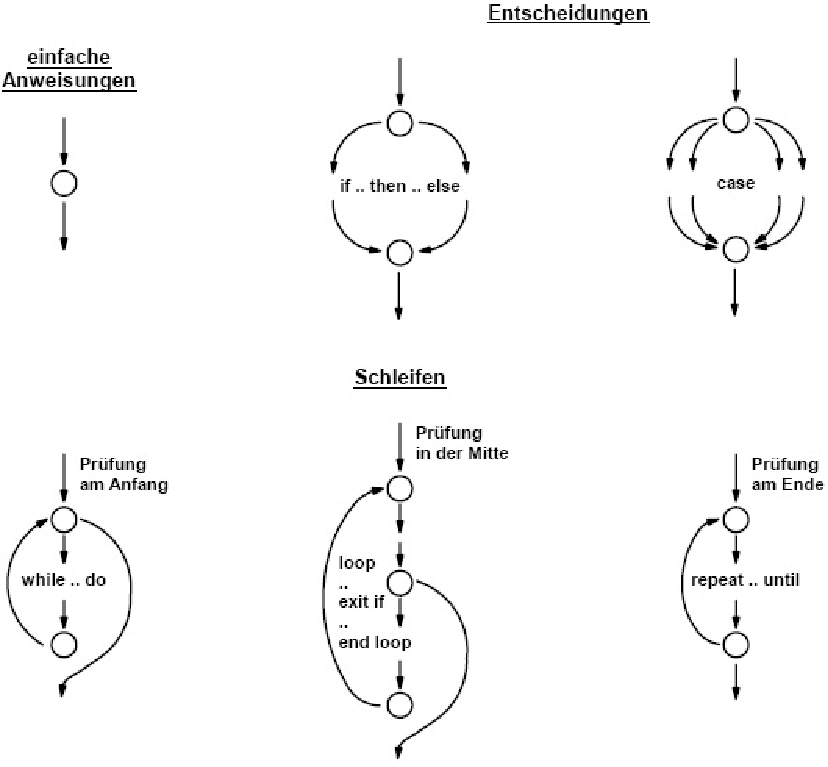
\includegraphics[width=0.75\textwidth]{bilder/Kontrollflussteile.pdf}
	\caption{Graphen f�r einzelne Konstrukte}
	\label{fig:Kontrollflussteile}
\end{figure}

Ein \textit{Segment} (Abbildung \ref{fig:segmente}) ist eine alternierende Folge von Knoten und Kanten mit maximaler L�nge, die folgende Eigenschaften besitzt:
\begin{itemize}
	\item Es gibt nur einen Eintrittspunkt (eingehende Kante) �ber den ersten Knoten des Segments.
	\item Wird der erste Knoten des Segments durchlaufen, so werden alle Knoten des Segments in der vorgesehenen Reihenfolge genau einmal durchlaufen.
\end{itemize}
\begin{figure}[h!]
	\centering
		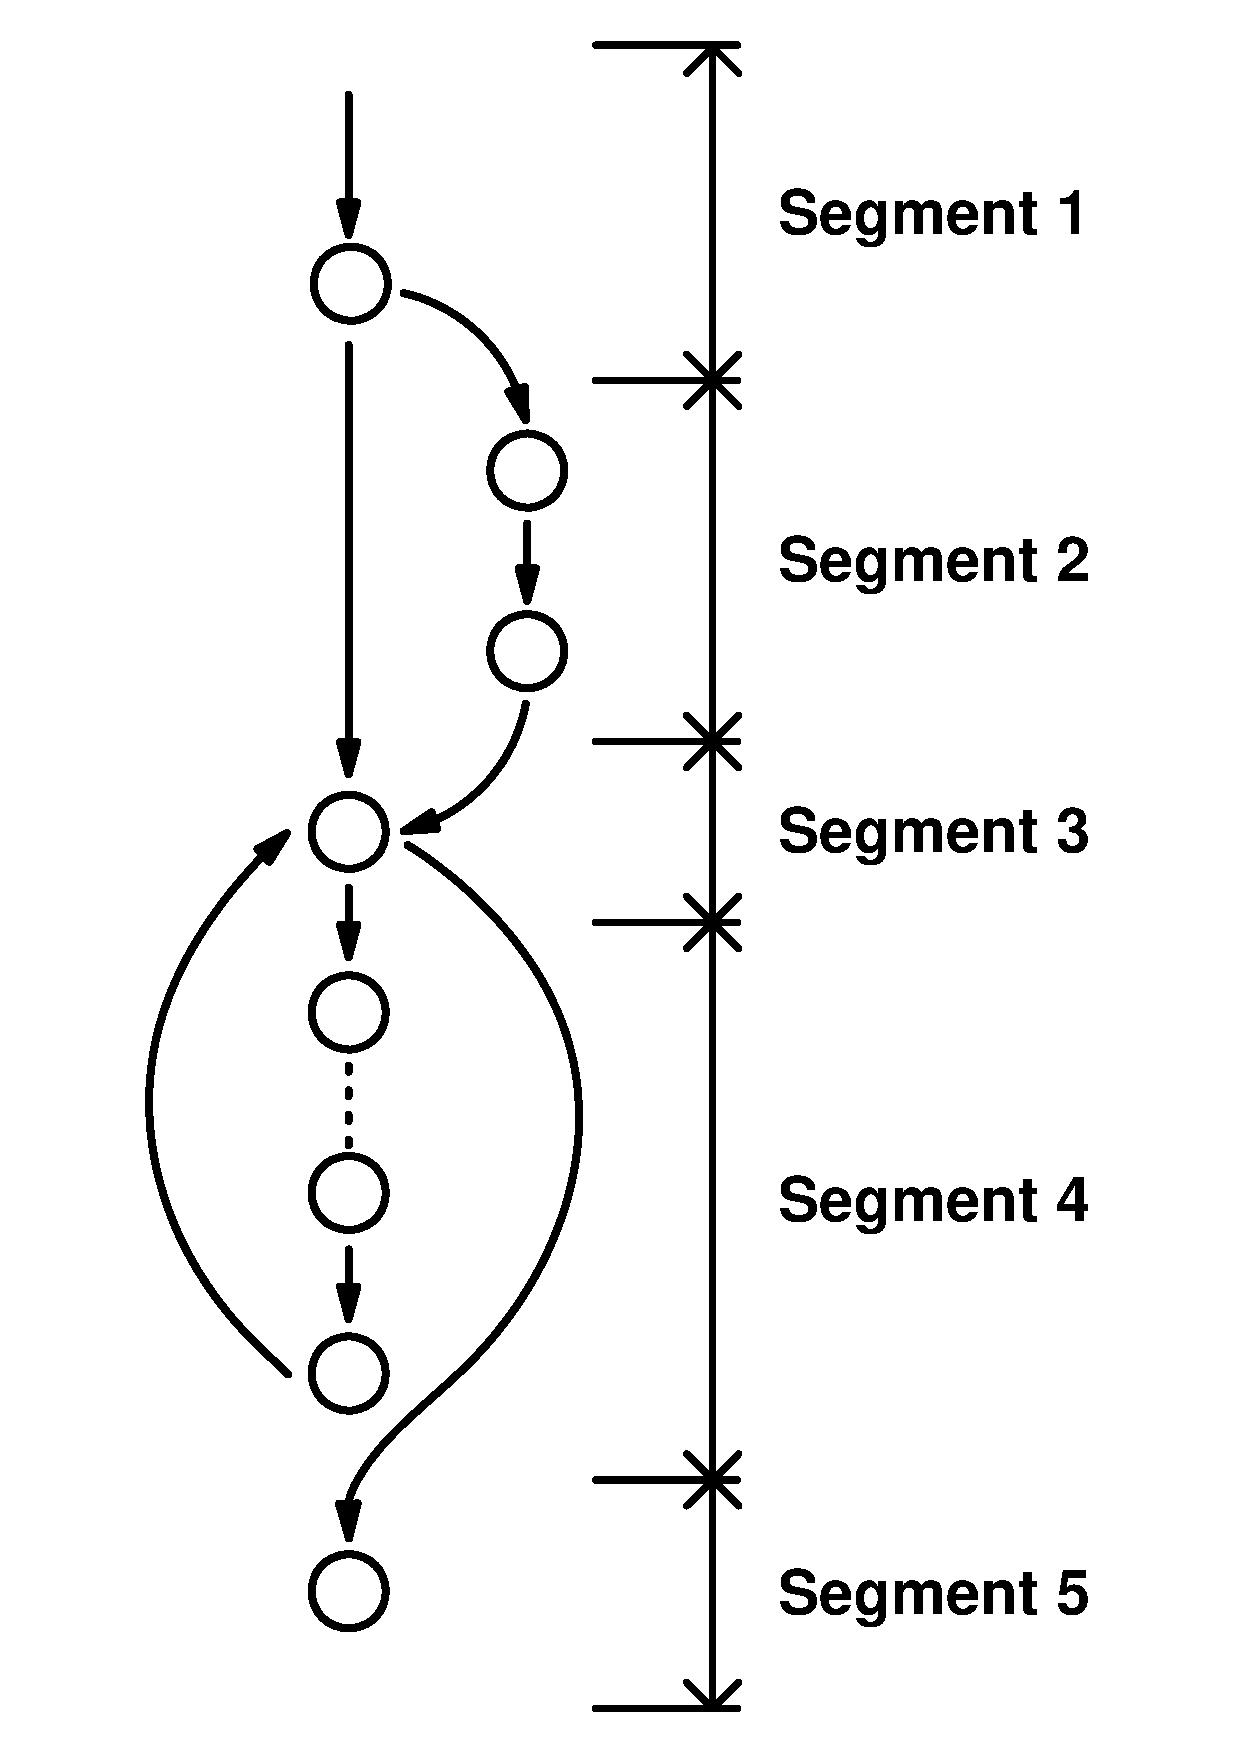
\includegraphics[width=0.4\textwidth]{bilder/segmente.pdf}
	\caption{Segmente in einem Kontrillflussgraph}
	\label{fig:segmente}
\end{figure}


Kontrollflu�graphen werden unter anderem f�r die Berechnung der logischen Komplexit�t eines Programmabschnitts und der kontrollflu�orientierten Abdeckungsmetriken.